\documentclass[8pt]{standalone}
\usepackage{pgfplots}
\pgfplotsset{compat=1.18}


\begin{document}
	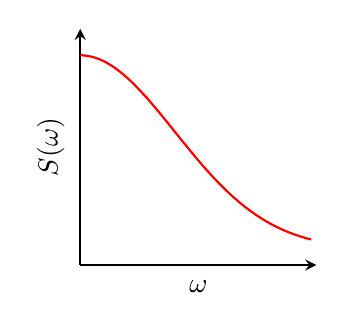
\begin{tikzpicture}
		\begin{axis}[
			width=3cm,
			height=3cm,
			xlabel={$\omega$},
			ylabel={$S(\omega)$},
			ytick=\empty,
			xtick=\empty,
			xmin=0, xmax=4.5,
			ymin=0, ymax=4.5,
			axis lines=left,
			axis line style={-stealth, thick, black},
			tick style={black, thick},
			scale only axis
			],
			
			\addplot[domain=0:4.4, samples=100, thick, red]{
				0.3 + 1/(0.108*sqrt(2 * pi)) * exp(-(x^2)/(60*0.108))
			};
		\end{axis}
	\end{tikzpicture}
\end{document}